	\subsection{Fully Depleted Silicon on Insulator (FD-SOI)}
	FD-SOI is a process technology that implements complementary metal oxide semiconductor (CMOS) transistors with an insulating layer of oxide, referred to as a burried oxide (BOX), between the channel of the transistors and the silicon substrate \cite{Planes2012}. The addition of such an oxide reduces capacitances of the fabricated transistors to the silicon substrate, resulting in lower overall capacitance than in bulk CMOS technologies. Thus higher frequency of operating is possible versus similar sized bulk process nodes. A further feature introduced by FD-SOI technology is the ability to form isolated wells beneath fabricated devices \cite{Wiatr2019}, which remain electrically isolated from the transistors via the BOX and from the substrate due to PN junctions inherent in well formation. This opens the possibility to achieve biasing across a wide voltage range of the regions below individual transistors (both for PMOS and NMOS devices), which enables tuning of individual transistor threshold voltages by exploitation of the MOS body effect. The well beneath a FD-SOI transistor is referred to as the "backgate". The implementation these features in the Global Foundaries 22FDX process is shown in figure \ref{fig:22fdx_wells}. 
	
			\begin{figure}[htb!]
			        \centering
			        \includegraphics[width=1\textwidth, angle=0]{./figs/theory/wiatr1-p4-wiatr-large}
			    \caption{22FDX cross-sectional construction of active devices \cite{Wiatr2019}.}
			    \label{fig:22fdx_wells}
			\end{figure}
	
	\subsection{MOSFET Models}

	\subsubsection{I-V relations}\label{sec:mos_iv}
	Basic models that describe the large signal current-voltage relations of a Metal Oxide Semiconductor Field Effect Transistor (MOSFET) are introduced here, based wholy from \cite{razavi_2017}. For the purposes of this work, a MOSFET is schematically represented in the manner of figure \ref{fig:mos_symbols}, with gate (G), drain (D), source (S) and backgate (B) terminals. Several operating regimes occur depending on the relation of the terminal voltages. Relevant to the scope of this work, are the linear, saturated and velocity saturated regions of MOSFET operation. Nominally, it is expected that when configured as in figure \ref{fig:vgs_sweep}, sweeping the gate-source voltage ($V_{GS}$), with the drain-source voltage ($V_{DS}$) set greater than 0 in the case of a NFET, that an increasing amount of current will enter the MOSFET drain after crossing a threshold voltage ($V_{TH}$). $V_{TH}$ is predominantly dependent of physical configuration of a FET (dimensions, doping, material), however is impacted by the backgate bias in what is termed "the body effect". A more detailed description of each operating regime will be given in the following discourse.

			\begin{figure}[htb!]
			        \centering
			        \includegraphics[width=0.5\textwidth, angle=0]{./figs/theory/fet_symbols}
			    \caption{MOSFET symbols.}
			    \label{fig:mos_symbols}
			\end{figure}

			\begin{figure}[htb!]
			        \centering
			        \includegraphics[width=0.8\textwidth, angle=0]{./figs/theory/vgs_sweep}
			    \caption{Drain current versus gate-source bias.}
			    \label{fig:vgs_sweep}
			\end{figure}


	% \textbf{Subthreshold Region}
	% $\xi$ is a factor of ideality, $V_T = k_B T/q$, where $k_B$ is the Boltzmann constant, T is the temperature in Kelvin, and $q$ represents the elementary charge.
	% \begin{equation}
	% 	I_D = I_0e^{\frac{V_{GS}}{\xi V_T}}
	% \end{equation}

	\textbf{Linear Region}
	Linear MOSFET operation occurs under the circumstances where  $|V_{GS}-V_{TH}| > |V_{DS}|$. The following equation is the I-V relation in this regime, where $\mu_n$ represents the electron mobility of the semiconductor in use (within the FET channel), $C_{ox}$ represents the MOS oxide capacitance. 
	\begin{equation}
		I_D = \mu_x C_{ox} \left(\frac{W}{L}\right)\left[(V_{GS}-V_{TH})V_{DS}-\frac{1}{2}V_{DS}^2\right]
	\end{equation}

	\textbf{Saturation Region}
	Saturation region occurs when $|V_{DS}| > |V_{GS}-V_{TH}|$. Notably, dependence of drain current on $V_{DS}$ is reduced, and in the case of the ideal models considered here, the effect of $V_{DS}$ are completely negated.
	\begin{equation}
		I_D = \frac{1}{2}\mu_n C_{ox} \left(\frac{W}{L}\right)(V_{GS}-V_{TH})^2
	\end{equation}


	\textbf{Velocity-saturation Region}
	In the scenario of high applied fields which arise in a short MOSFET channels, carrier velocity can saturate to a limited velocity, $v_{sat}$. The point at which this effect takes place is device dependent. For approximate consideration it can be understood to occur when $|V_{DS}/L > E_{crit}|$, where $E_{crit}$ is the electric field which the carrier velocity-electric field relation ($v = \mu E$) of the channel semiconductor becomes sub-linear. Below is the MOSFET model under such circumstances.
	\begin{equation}
		I_D = WC_{ox}(V_{GS}-V_{TH})v_{sat}
	\end{equation}

	\subsubsection{Body Effect}
	Application of a bias to the substrate below a bulk MOSFET, or to the well below a FD-SOI MOSFET, has a direct effect on the threshold voltage of a MOSFET. For a bulk MOSFET, change of body bias affects the width of source-drain and source-body depletions, which consequently can increase or decrease the magnitude of the channel depletion charge as seen by the gate terminal needed to achieve channel inversion. This corresponds to a differential in the threshold voltage. The below equation \cite{razavi_2017} quantifies this effect for bulk devices. $\gamma$ is the body effect coefficient, $2\Phi_F$ represents the MOS surface potential. $V_{TH}$ is non-linearly related to the source-body voltage $V_{SB}$.
	\begin{equation}
		V_{TH} = V_{TH0} + \gamma\left( \sqrt{2\Phi_F + V_{SB}} - \sqrt{|2\Phi_F|} \right)
	\end{equation}
	In the case of FD-SOI transistors, the nature of the body effect is modified due to the presence of the BOX. Thus, an approximate derivation for body effect will be provided here. In FD-SOI, the active channel region is thin, and under strong inversion, the entire channel region is depleted of charge. Supposing a channel height Z and channel doping $N_A$, the total charge to deplete the channel for inversion to occur is $Q_{d} = N_AZ$. With oxide capacitance $C_{ox,fg}$ associated with the front gate, the portion of the threshold voltage associated with total depletion of the channel is, from the front gate perspective:
	\begin{equation}
		V_{d,fg} = \frac{Q_d}{C_{ox,fg}} = \frac{N_AZ}{C_{ox,fg}} 
	\end{equation}
	Supposing that the back gate has capacitance of $C_{ox,bg}$, with bias applied $V_{BS}$, the back gate can be seen to "rob" the front gate of $Q_{bg} = C_{ox,bg}V_{BS}$ when in inversion. Thus results in a partial change of the front gate referred voltage required to obtain channel depletion:
	\begin{equation}
		V_{d,fg}^{'} = \frac{Q_d-Q_{bg}}{C_{ox,fg}} = \frac{Q_d}{C_{ox,fg}} - \frac{C_{ox,bg}}{C_{ox,fg}}V_{BS} = V_{d,fg}-\Delta V_{th,bg}
	\end{equation}
	It is noted that this can be writen as the nominal value of $V_{d,fg}$ minus a differential. This differential is the resulting change in threshold voltage due to back gate bias, $\Delta V_{th,bg}$:
	\begin{equation}
		\Delta V_{th,bg}= \frac{C_{ox,bg}}{C_{ox,fg}}V_{BS} 
	\end{equation}	
	This is linear with applied back gate bias, and that the strength of the coupling is tunable by the ratio of front gate and back gate capacitances. Typically this ratio is $<<1$. If we define the body effect coefficient $\gamma$ as:
	\begin{equation}
		\gamma = \frac{C_{ox,bg}}{C_{ox,fg}}
	\end{equation}
	Given a nominal threshold voltage of $V_{TH0}$, in FD-SOI, the threshold voltage can be represented as:
	\begin{equation}\label{eq:body_effect}
		V_{TH} = V_{TH0} - \gamma V_{BS}
	\end{equation}

	\subsubsection{Linearization of MOSFET models}
	Under conditions where a MOSFET is held at near constant bias levels, with only minor variations around the DC operating level, simpler linearized models of the transistors can be developed. For the different operating regions of the MOSFET, the I-V relations can be generalized in terms of the function $I_D(V_{GS}, V_{DS}, V_{BS})$. Linearization is then obtained by calculating the slope of $I_D$ with respect to the potentials $V_{GS}, V_{DS}, V_{BS}$. The resulting parameters (given as equations \ref{eq:gm} to \ref{eq:fet_out_r}) are the transconductance $g_m$, relating gate drive to drain current, transconductance $g_{mb}$, relating body drive to drain current, and resistance $r_o$, relating drain voltage to drain current. Due to linearization, the current contributions are superimposed to determine total drain current. The linearized circuit which replaces the four terminal MOSFET symbols of figure \ref{fig:mos_symbols} is given by the linearized circuit of figure \ref{fig:ss_model}.

	\begin{align}
		g_m & = \frac{\partial }{\partial V_{GS}}I_D(V_{GS}, V_{DS}, V_{BS}) \label{eq:gm}\\
		g_{mb} & = \frac{\partial }{\partial V_{BS}}I_D(V_{GS}, V_{DS}, V_{BS})\\
		r_o &= \left(\frac{\partial }{\partial V_{DS}}I_D(V_{GS}, V_{DS}, V_{BS})\right)^{-1}\label{eq:fet_out_r}
	\end{align}
		\begin{figure}[htb!]
		        \centering
		        \includegraphics[width=1\textwidth, angle=0]{./figs/theory/lin_oppoint}
		    \caption{Transconductances as slope localized at operating point of I-V curve.}
		    \label{fig:lin_oppoint}
		\end{figure}

		\begin{figure}[htb!]
		        \centering
		        \includegraphics[width=0.4\textwidth, angle=0]{./figs/theory/ss_model}
		    \caption{Linearized (small-signal) MOSFET model.}
		    \label{fig:ss_model}
		\end{figure}
		\FloatBarrier
	A useful relation based on this linearization can be determined, based on the FD-SOI body effect equation \ref{eq:body_effect}, and the I-V relations for the three MOSFET operation regions discussed in section \ref{sec:mos_iv}. Computation of $g_{m}$ and $g_{mb}$ for all three regions with the FD-SOI body effect yields the same result given in equation \ref{eq:gm_gmb_relation}. This is that $g_{mb}$ and $g_{m}$ are related by the body effect coefficient $\gamma$.
	\begin{equation}\label{eq:gm_gmb_relation}
	g_{mb} = \gamma g_{m}
	\end{equation}

		



	\subsection{Basic PLL}
	A phase locked loop (PLL) is a feedback system whose output tracks or maintains a fixed phase relationship to an input signal. PLLs are well suited for frequency synthesis, which is the process of generating derivative frequencies from some reference frequency. Given a reference signal with phase trajectory $\Phi_{ref}$ and output signal with phase $\Phi_{out}$, a PLL can be modeled as in figure \ref{fig:basic_fb} using an elementary feedback system, with feedforward and feedback networks A(s) and B(s). 
	\begin{figure}[htb!]
		\center\include{./figs/basic_feedback}
		\caption{Phase locked loop as elementary feedback system.}
		\label{fig:basic_fb}
	\end{figure}
	\FloatBarrier
	The closed loop phase response for $\Phi_{ref}$ to $\Phi_{out}$ is therefore:
	\begin{equation}
		\frac{\Phi_{out}(s)}{\Phi_{ref}(s)} = \frac{A(s)}{1+A(s)B(s)}
	\end{equation}
	A case of interest is when B(s) = 1/N, where N is a constant, and the loop gain L(s) = A(s)B(s) $>>$ 1. The closed loop response for this case is:
	\begin{equation}\label{mult_by_n}
		\frac{\Phi_{out}(s)}{\Phi_{ref}(s)} \approx \frac{A(s)}{A(s)B(s)} = \frac{1}{B(s)} = N
	\end{equation}
	We see that the phase through the PLL is multiplied by a factor of N. If the input phase signal is sinusoidal with frequency $\omega_{ref}$, and likewise the output with $\omega_{out}$, then $\phi_{ref}(t)=\omega_{ref}t$ and $\phi_{out}(t)=\omega_{out}t$. Accordingly:
	\begin{equation}
		\frac{\Phi_{out}(t)}{\Phi_{ref}(t)} = \frac{\omega_{out}t}{\omega_{ref}t} \approx N \hspace{1em} \rightarrow \hspace{1em} \omega_{out} \approx N\omega_{ref}
	\end{equation}
	Therefore, it is observed that a PLL allows for the generation of a new frequency from a reference frequency signal, which is termed as "frequency synthesis". With a feedback division ratio of 1/N, the PLL multiplies the reference frequency by a factor of N. Hereon, the B(s) portion of a PLL feedback network is referred to as a divider, with associated division raito N.

	\subsection{PLL Synthesizer Architecture}
		A typical architecture for implementing a physically realizable PLL frequency synthesizer \cite{Razavi1996DesignOM} is shown in figure \ref{fig:basic_pll}. This PLL is comprised of four components: (1) a phase detector, herein PD, (2) a loop filter, herein H$_{LF}$(s), (3) a voltage controlled oscillator, herein VCO, and (4) a divider, indicated as "$\div$ N" in figure \ref{fig:basic_pll}. In control systems parlance, the loop filter corresponds to a controller, the VCO an actuator, and the divider as feedback.
		\begin{figure}[htb!]
			\center\fontfamily{\sfdefault}\selectfont
% XCircuit output "basic_pll.tex" for LaTeX input from basic_pll.ps
\def\putbox#1#2#3#4{\makebox[0.00000in][l]{\makebox[#1][l]{}\raisebox{\baselineskip}[0.00000in][0.00000in]{\raisebox{#2}[0.00000in][0.00000in]{\scalebox{#3}{#4}}}}}
\def\rightbox#1{\makebox[0.00000in][r]{#1}}
\def\centbox#1{\makebox[0.00000in]{#1}}
\def\topbox#1{\raisebox{-0.60\baselineskip}[0.00000in][0.00000in]{#1}}
\def\midbox#1{\raisebox{-0.20\baselineskip}[0.00000in][0.00000in]{#1}}
   \scalebox{1}{
   \normalsize
   \parbox{4.66667in}{
   \includegraphics[scale=0.70000]{./figs/basic_pll.pdf}\\
   % translate x=344 y=640 scale 0.38
   \putbox{1.05700in}{1.37900in}{1.20}{PD}%
   \putbox{2.42900in}{0.56700in}{1.20}{$\div$ N}%
   \putbox{0.42000in}{1.52600in}{1.20}{$\Phi_{ref}$}%
   \putbox{3.80100in}{1.52600in}{1.20}{$\Phi_{out}$}%
   \putbox{1.99500in}{1.37900in}{1.20}{H$_{LF}$(s)}%
   \putbox{3.15700in}{1.37900in}{1.20}{VCO}%
   \putbox{1.58200in}{0.70700in}{1.20}{$\Phi_{div}$}%
   \putbox{1.56800in}{1.52600in}{1.20}{$\Phi_e$}%
   \putbox{2.63200in}{1.52600in}{1.20}{V$_{ctrl}$}%
   } % close 'parbox'
   } % close 'scalebox'
   \vspace{-\baselineskip} % this is not necessary, but looks better
\fontfamily{\rmdefault}\selectfont

			\caption{High-level PLL Synthesizer Architecture.}
			\label{fig:basic_pll}
		\end{figure}
		\FloatBarrier
		Further explaination of these components will be hereafter made.

		\subsubsection{Phase Detector}
		A phase detector acts as the summation point of figure \ref{fig:basic_fb}, which measures the phase error $\Phi_e$ between the reference signal and the output of the PLL. The phase error is then used by the controller, which is implemented as the loop filter, to adjust the PLL's state. Such a phase detector may also have intrinsic gain, given by $K_{PD}$.
		\begin{equation}
			\Phi_e(s) = K_{PD}(\Phi_{ref}(s) - \Phi_{div}(s))
		\end{equation}

		\subsubsection{Bang-bang phase detector}\label{bbpd_theory}
		% First reference : \cite{toifl_1998}

		\begin{figure}[htb!]
		    \centering
		    \begin{subfigure}{0.5\textwidth}
		        \centering
		        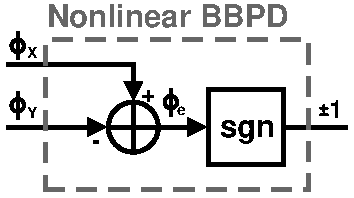
\includegraphics[width=0.75\textwidth, angle=0]{./figs/theory/bbpd_nonlinear}
		        \caption{ }
		        \label{fig:bbpd_nonlinear}
		    \end{subfigure}%
		    \begin{subfigure}{0.5\textwidth}
		        \centering
		        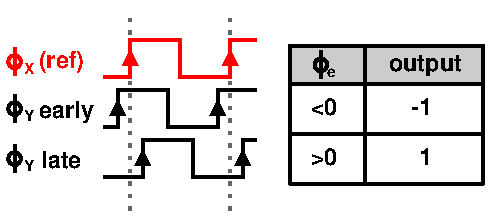
\includegraphics[width=1\textwidth, angle=0]{./figs/theory/bbpd_timing}
		        \caption{ }
		        \label{fig:bbpd_timing}
		    \end{subfigure}
		    % \caption{x.}

		    \caption{\textbf{(a)} BBPD schematic, \textbf{(b)} BBPD timing.}
		    \label{fig:bbpd_theory}
		\end{figure} 
			A simple implementation of a phase detector is a bang-bang phase detector (BBPD) \cite{zanuso_2009}. As exhibited in figure \ref{fig:bbpd_theory}, a BBPD outputs a value of 1 if the input $\Phi_Y$ is late relative to the reference $\Phi_X$ (representing a clock signal), and -1 if it is early. A BBPD shows abrupt nonlinearity in its transfer characteristics. If the error signal variance $\sigma_{\Phi_e}^2$ is constant, which is expected in steady-state PLL operation, a linearized model for phase detector gain can be established \cite{xu_abidi_2017}, given in equation \ref{eq:nom_bbpd_gain}.

			A linearized version of the BBPD is illustrated in figure \ref{fig:bbpd_linearized}. The output $\mathrm{z}$ valued as $\pm 1$ (its variance $\sigma_y^2$=1).
			\begin{equation}\label{eq:nom_bbpd_gain}
				K_{BBPD} = \frac{\mathbb{E}[\Phi_e(t)\cdot\mathrm{z}(t)]}{\mathbb{E}[\Phi_e^2(t)]} = \sqrt{\frac{2}{\pi}}\frac{1}{\sigma_{\Phi_e}}
			\end{equation}
			\begin{figure}[htb!]
				\center\includegraphics[width=0.4\textwidth, angle=0]{./figs/theory/bbpd_linearized}
				\caption{Linearized bang-bang phase detector.}
				\label{fig:bbpd_linearized}
			\end{figure}

			\subsubsection{BBPD Noise}\label{sec:bbpd_noise}
			Given the output of the BBPD is of fixed power $\sigma_z^2$ = 1, a linearized gain of $K_{BBPD}$, a phase error power of $\mathrm{Var}[\Phi_e(t)] = \sigma_{\Phi_e}^2$, and $\mathbb{E}[\Phi_e(t)]=0$, the noise power  $\sigma_{n_{BBPD}}^2$ out of the BBPD is in equation \ref{eq:bbpd_gain}. $K_{BBPD}^2\sigma_{\Phi_e}^2$ represents the power of the phase error signal component post-detector, and it is assumed that noise power and signal power are uncorrelated.
			\begin{equation}\label{eq:bbpd_gain}
				\sigma_{n_{BBPD}}^2 = \sigma_z^2 - K_{BBPD}^2\sigma_{\Phi_e}^2 = 1-\frac{2}{\pi}
			\end{equation}


			Observe that the BBPD noise power is constant. If the reference signal is a clock signal with frequency $f_{ref}$, the BBPD noise spectral density is in equation \ref{eq:bbpd_noise_psd}.
			\begin{equation}\label{eq:bbpd_noise_psd}
				S_{ n_{BBPD}(f)} = \frac{\sigma_{n_{BBPD}}^2}{\Delta f} = \frac{\left(1-\frac{2}{\pi}\right)}{f_{ref}}
			\end{equation}



		\subsubsection{Divider}
			A divider is used as the feedback path in the PLL, where the division ratio N controls the frequency multiplication of a PLL synthesizer. The transfer function of the divider is:
			\begin{equation}
				\mathrm{H}_{div}(s) = \frac{\Phi_{div}(s)}{\Phi_{out}(s)} = \frac{1}{\mathrm{N}}
			\end{equation}


			Dividers are commonly realized as digital modulo-N counters that count oscillation cycles \cite{weste_harris_2011}. With a division ratio of N, the output of the divider will have an active edge transition (considered to be rising edge as shown in figure \ref{fig:digital_div}) every N input cycles. Phase information is inferred from the output edge timing, which occurs with time interval N$/f_{osc}$, and is equal to the point at which output phase equals a multiple of $2\pi$. Thus a digital divider does not provider continuous phase information, but rather a sampled phase signal with rate $f_{osc}/$N. 
			\begin{figure}[htb!]
				\center\include{./figs/digital_div}
				\caption{Digital divider signals.}
				\label{fig:digital_div}
			\end{figure}


		\subsubsection{Loop Filter}
			A loop filter behaves as the controller of a PLL, namely controlling the phase-frequency response of PLL. The choice of loop filter transfer function significatly affects transient PLL behavior, as well as phase noise performance, as is later described. Here, a pole-zero based controller is defined for use in this work. This is designed to have P poles and Z zeros, and can be represented in the canonical form of equation \ref{eq:lf_general_form} as a rational function of polynomials of s with coefficients given with $\{a_0, ..., a_P\}$ and $\{b_0, ..., b_Z\}$.
			\begin{equation} \label{eq:lf_general_form}
				\textnormal{H}_{LF}(s) = \frac{\sum_{j=0}^Z b_js^j}{\sum_{k=0}^P a_ks^k}
			\end{equation}
			
		\subsubsection{Loop Filter Discretization and Digitization}\label{lf-discretization}
			In PLLs which sample on a fixed interval defined by a reference clock frequency $f_{ref}$, derivation of a discrete time controller model is necessary. This is derived from the general form continuous loop filter (equation \ref{eq:lf_general_form}) via application of a continous s-domain to discrete z-domain transformation. Strictly speaking, $z^{-1} = e^{-s\Delta T_s}$ for values on the unit circle, i.e. r=1 \cite{proakis_1993_z}. If the PLL sampling rate $f_s$=$f_{ref}$ is constrained to be sufficiently higher than the implemented filter bandwidth (i.e. PLL loop bandwidth, $BW_{loop}$), a simpler transformation using a truncated Taylor series approximation is applicable. Given the $1/\Delta T_s$=$f_{s}$ as the relation for sampling rate, then:
			\begin{align*}
				z^{-1} &= e^{-s\Delta T_s} && \text{(definition of z on unit circle)} \\
				&= \sum_{k=0}^\infty\frac{(-s\Delta T_s)^k}{k!} && \text{(exponential Taylor series)} \\
				&\approx 1-s\Delta T_s &&\text{(if $|s\Delta T_s| = 2\pi\mathrm{BW}_{loop}\cdot \Delta T_s << 1$)} \\
			\end{align*}
			Thus the s-to-z and z-to-s identities for the approximate transform are:
			\begin{align}
				z^{-1} &= 1-s\Delta T_s\\
				s &= \frac{1}{\Delta T_s}(1-z^{-1}) \label{eq:s_to_z_xfrm}
			\end{align}
			Applying equation \ref{eq:s_to_z_xfrm} to the general loop filter of equation \ref{eq:lf_general_form} yields the z-domain loop filter:
			\begin{align}
				\textnormal{H}_{LF}(z) &= \left.\textnormal{H}_{LF}(s)\right\vert_{s=\frac{1}{\Delta T_s}(1-z^{-1})} = \left.\frac{\sum_{j=0}^Z b_js^j}{\sum_{k=0}^P a_ks^k}\right\vert_{s=\frac{1}{\Delta T_s}(1-z^{-1})}\\
				&= \frac{\sum_{j=0}^Z \frac{b_j}{\Delta T_s^j}(1-z^{-1})^j}{\sum_{k=0}^P \frac{a_k}{\Delta T_k}(1-z^{-1})^k} \label{eq:z_general_lf}
			\end{align}
			Equation \ref{eq:z_general_lf} is transformed into a digitally implementable form by reorganizing into the canonical representation of equation \ref{eq:canonical_z_tf}, which then determines the tap coefficients for the sampled-time difference equation in equation \ref{eq:cananical_diff_eq}. 
			\begin{align}
				\textnormal{H}_{LF}(z) &= \frac{\sum_{j=0}^P b_j^{'}z^{-j}}{1+\sum_{k=1}^Z a_k^{'}z^{-k}}\label{eq:canonical_z_tf} \\
				y[n]&= -\sum_{k=1}^P a_k^{'}y[n-k] + \sum_{j=0}^Z b_j^{'}x[n-j] \label{eq:cananical_diff_eq}
			\end{align}
			The obtained difference equation is directly implementable in digital hardware with a direct form-I IIR filter \cite{proakis_1993} shown in figure \ref{fig:filt_implementation}. Such a design is a cantidate for automatic synthesis of digital logic. The filter coefficients $\{a_1^{'}, ..., a_P^{'}\}$ and $\{b_0^{'}, ..., b_Z^{'}\}$ must be quantized into finite resolution fixed point words for a complete digital implementation. The delay elements ($z^{-1}$ blocks) are implementable digitally as registers, the coefficient gains are implementable with array multipliers, and the adders are implementable with digital adders.
			\begin{figure}[htb!]
				\center\include{./figs/direct_type_1_primed}
				\caption{Direct form I implementation of IIR filter.}
				\label{fig:filt_implementation}
			\end{figure}


			
		\subsubsection{Voltage/Digitally Controlled Oscillator}
			A controlled oscillator is an oscillator with frequency controlled by an input signal. When this input signal takes the form of an analog voltage $\textnormal{V}_{ctrl}$, it is referred to as a voltage controlled oscillator (VCO). Otherwise, when controlled digitally with an oscillator tuning word (OTW) u[n], it is referred to as a digitally controlled oscillator (DCO). Nominally, a controlled oscillator is characterized by its gain, in the case of a VCO is $K_{VCO} = \partial f/\partial \textnormal{V}_{ctrl}$. With a DCO, the gain is $K_{DCO} = \Delta f/LSB$, that is the change in frequency per least significant bit. Analyzed in terms of phase (for the VCO case), an oscillator can be seen as a time-phase integrator, provided a nominal oscillator frequency of $f_0$:
			\begin{equation}\label{eq:vco_ph}
				\Phi_{VCO}(t) = \Phi_{out}(t) = \int2\pi(K_{VCO}\textnormal{V}_{ctrl}(t) + f_0)\mathrm{dt}
			\end{equation}
			In the s-domain, the transfer function for a VCO is in equation \ref{eq:vco_tf} and equation \ref{eq:dco_tf} for a DCO. 
			\begin{equation}\label{eq:vco_tf}
				\mathrm{H}_{VCO}(s) = \frac{\Phi_{VCO}(s)}{\textnormal{V}_{ctrl}(s)} = \frac{2\pi K_{VCO}}{s}
			\end{equation}
			\begin{equation}\label{eq:dco_tf}
				\mathrm{H}_{DCO}(s) = \frac{\Phi_{VCO}(s)}{\textnormal{u}(s)} =  \frac{2\pi K_{DCO}}{s}
			\end{equation}
			By application of discretization and conversion to difference equations, the sampled-time oscillator phase signals are equation \ref{eq:vco_ph_de} for a VCO and equation \ref{eq:dco_ph_de} for a DCO. 
			\begin{equation}\label{eq:vco_ph_de}
				\Phi_{out}[n] = \Phi_{out}[n-1] + 2\pi K_{VCO}\Delta T_s\textnormal{V}_{ctrl}[n]
			\end{equation}
			\begin{equation}\label{eq:dco_ph_de}
				\Phi_{out}[n] = \Phi_{out}[n-1] + 2\pi K_{DCO}\Delta T_su[n]
			\end{equation}

		\subsubsection{Closed Loop PLL Transfer Function}\label{cont_pll_tf}
			With a PLL described at the component level, the closed loop dynamics of the PLL can be computed. A PLL loop gain L(s) can be first determined (using BBPD definition for phase detector gain). 
			\begin{equation}
				\mathrm{L}(s) = K_{PD}\textnormal{H}_{LF}(s)\textnormal{H}_{DCO}(s)\textnormal{H}_{div}(s) = \frac{2\pi K_{PD}K_{DCO}}{\mathrm{N}}\frac{1}{s}\frac{\sum_{j=0}^Z b_js^j}{\sum_{k=0}^P a_ks^k}
			\end{equation}
			Closing the loop with the phase detector as the feedback summation point, the response of the PLL from reference to output is in equation \ref{eq:cont_pll_tf}.
			\begin{align} \label{eq:cont_pll_tf}
				\mathrm{T}(s) = \frac{\Phi_{out}(s)}{\Phi_{ref}(s)} = \frac{2\pi K_{PD}K_{DCO}\sum_{j=0}^Z b_js^j}{\sum_{k=0}^P a_ks^{k+1} + \frac{2\pi K_{PD}K_{DCO}}{\mathrm{N}}\sum_{j=0}^Z b_js^j} = \mathrm{N}\frac{\mathrm{L}(s)}{1 + \mathrm{L}(s)}
			\end{align}



	%%%%%%%%%%%%%%%%%%%%%%%%%%%%%%%%%%%%%%%%%%%%%%%%%%%%%%%%%%%%%%%%%%%%%%%%%%%%%%%%%%%%%
	\subsection{Phase noise}
		Phase noise can be described as undesired variation in an oscillator's phase trajectory from ideal. If an oscillator's frequency is $\omega_{osc}$, then with additive phase noise, the phase of an oscillator is in \ref{eq:osc_ph_traj}. 
		\begin{equation}\label{eq:osc_ph_traj}
			\Phi_{osc}(t) = \omega_{osc}t + \Phi_n(t)
		\end{equation}
		This is composed of a linear phase component $\omega_{osc}t$ and a noise component $\Phi_n(t)$. In the frequency domain, the effect of phase noise is that it broadens the tone of the oscillator, as shown in figure \ref{fig:phase_noise_psd}. Phase noise can be viewed as instability in terms of oscillator frequency.
		\begin{figure}[htb!]
	        \centering
	        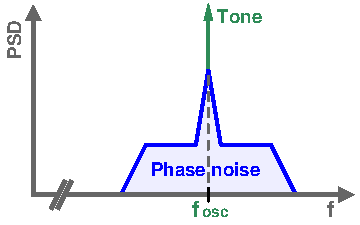
\includegraphics[width=0.5\textwidth, angle=0]{./figs/theory/phase_noise_psd}
		    \caption{Effect of phase noise on frequency tone.}
		    \label{fig:phase_noise_psd}
		\end{figure}

		\subsubsection{Relation to Power spectral density}\label{sec:pn_to_psd}
		An oscillator's voltage waveform can be described in terms of a phase trajectory function $\Phi_{osc}(t)$ and amplitude $A_0$ in the following manner (ignoring higher harmonics):
		\begin{equation}\label{eq:osc_wfm}
			V_{osc}(t) = \Re\left\{A_0e^{j\Phi_{osc}(t)}\right\}
		\end{equation}
		 In an oscillator, it is desirable for phase noise to be small, and zero mean ($\mathbb{E}[\Phi_{n}(t)]=0$). Using a constraint $\mathrm{Var}[\Phi_{n}(t)] << 1$ the following approximations can be applied to determine the oscillators spectral density in terms of the phase noise component $\Phi_n(t)$.
		\begin{align}
			V_{osc}(t) &= \Re\left\{A_0e^{j\omega_{osc}t}e^{j\Phi_{n}(t)}\right\} && \text{(oscillator waveform)} \\
			&= \Re\left\{A_0e^{j\omega_{osc}t}\sum_{k=0}^\infty\frac{(j\Phi_{n}(t))^k}{k!}\right\} && \text{(apply exponential Taylor series)} \\
			&\approx  \Re\left\{A_0e^{j\omega_{osc}t} +j\Phi_{n}(t)A_0e^{j\omega_{osc}t}\right\} && \text{(truncate series at k=1 given $\mathrm{Var}[\Phi_{n}(t)] << 1$)} \\
			&= A_0\cos(\omega_{osc}t) - \Phi_{n}(t)A_0\sin(\omega_{osc}t) &&\text{(taking real component)}\label{eq:pll_out_approx}\\
		\end{align}
		The result is a carrier cosine signal, and an orthogonal sine signal modulated by the phase noise $\Phi_{n}$. From this, the spectral density of the phase noise relative to the carrier can be estimated. The power spectral density $S_{V_{osc}}$ is computed in equations \ref{eq:psd_vout}-\ref{eq:psd_noise}. Due to orthogonality of the sine/cosine components of equation \ref{eq:pll_out_approx}, the cross terms that appear in the PSD computation are zero. 
		\begin{align}
			S_{V_{out}}(f) =& \lim_{\Delta T\rightarrow\infty}\frac{1}{\Delta T}|\mathcal{F}\{V_{out}(t)\cdot\mathrm{rect}(t/\Delta T)\}|^2 \label{eq:psd_vout}\\
			=&\lim_{\Delta T\rightarrow\infty}\frac{A_0^2}{\Delta T}|\mathcal{F}\{\cos(\omega_{osc}t)\cdot\mathrm{rect}(t/\Delta T)\}|^2 \label{eq:psd_carrier}\\ 
			&+ \lim_{\Delta T\rightarrow\infty}\frac{A_0^2}{\Delta T}|\mathcal{F}\{\Phi_{n}(t)\cdot\mathrm{rect}(t/\Delta T)\}*\mathcal{F}\{\sin(\omega_{osc}t)\cdot\mathrm{rect}(t/\Delta T)\}|^2 \label{eq:psd_noise}\\
		\end{align}
		 The noise power spectral density function of the output waveform $\mathcal{L}(\Delta f)$ is defined as the noise PSD at offset $\Delta f$ from the carrier frequency $f_{osc}$, normalized to the carrier power. Here the PSD of the carrier component is given by equation \ref{eq:psd_carrier}, and the noise component by equation \ref{eq:psd_noise}. Shifting equation \ref{eq:psd_noise} by $-\omega_{osc}$ and performing normalization for carrier power results in:
		\begin{equation}\label{eq:pn_psd_relation}
			\mathcal{L}(\Delta f) = \left.\lim_{\Delta T\rightarrow\infty}\frac{1}{\Delta T}|\mathcal{F}\{\Phi_{n}(t)\cdot\mathrm{rect}(t/\Delta T)\}|^2 \right|_{f=\Delta f}= S_{\Phi_{n}}(\Delta f)
		\end{equation}

		Thus, the noise PSD $\mathcal{L}(\Delta f)$ of the PLL output waveform relative to the carrier is equal to the PSD of the phase noise signal $\Phi_{n}(t)$, provided $\text{Var}[\Phi_{n}(t)] << 1$. The PSD of $\Phi_{n}(t)$ is notated as $S_{\Phi_{n}}(\Delta f)$.


	\subsubsection{Leeson's model}\label{dco_noise}
		Oscillator noise from thermal and stochastic sources is typical represented mathematically using Leeson's model for oscillator phase noise \cite{leeson_1966}. Leeson's model considers noise power density at an offset $\Delta f$ from the oscillator tone (carrier). Noise power density is represented with the function $\mathcal{L}(\Delta f)$, which is the noise power density normalized to the power of the oscillator carrier tone, in other words in units of dBc/Hz. Leeson's model divides phase noise into three regions, illustrated in figure \ref{fig:leeson_pn}: (1) flicker-noise dominated, with a slope of -30 dB/decade, (2) white frequency-noise dominated, with -20 dB per decade, and (3) a flat region, limited by the thermal noise floor or amplitude noise. It is noted that phase noise components are at frequencies different than the carrier, hence are orthogonal, and can be treated as independent components that are added to the main oscillator tone signal for analysis. 

			\begin{figure}[htb!]
		        \centering
		        \include{./figs/leeson_pn}
			    \caption{Phase noise regions of Leeson's model.}
			    \label{fig:leeson_pn}
			\end{figure}

		The equation for $\mathcal{L}(\Delta f)$ (from \cite{lee_hajimiri_2000}) is in equation \ref{eq:leesons}, and is dependent on temperature T, excess noise factor F, DC oscillator power $P_{DC}$, oscillator Q factor, and the transition frequencies $f_1$ and $f_2$ that separate the different noise regions. It is of interest to note that the phase noise relative to the carrier will increase as power decreases, which provides challenge for creating low power oscillators with acceptable phase noise characteristics. 
		\begin{equation}\label{eq:leesons}
		\mathcal{L}(\Delta f) = 10\log_{10}\left[\frac{2\text{F}k_B\text{T}}{P_{DC}}\left(1+\left(\frac{f_2}{2Q\Delta f}\right)^2\right)\left(1+\frac{f_1}{|\Delta f|}\right)\right] = S_{\Phi n_{DCO}}(\Delta f)
		\end{equation}
		For notational consistency, the following redefinition is used in the remainder of this paper: $S_{\Phi n_{DCO}}(f) = \mathcal{L}(\Delta f)|_{\Delta f = f}$

	\subsubsection{Phase Noise Figures of Merit}
	A common method to assign a figure of merit (FOM) to oscillator phase noise performance is to utilize the below relation \cite{Kinget1999}. Such a model assumes linear tradeoffs between power, frequency, and phase noise, and assumes that the rolloff of phase noise will occur with -20 dB/decade. A Lower FOM here is better.
	\begin{equation}\label{eq:fom_pn}
		\textnormal{FOM}_{\textnormal{pn}} = 10\log_{10}\left(\frac{P_{DC}}{\textnormal{1 mW}}\cdot\left(\frac{\Delta f}{f_0}\right)^2\right) + \mathcal{L}(\Delta f)
	\end{equation}
	Another FOM applied to PLLs is provided below, based on the RMS jitter of the PLL \cite{XiangGao2009}. Here, RMS jitter is used as the phase spectrum of a PLL is often more complicated than a simple oscillator, containing spurs, in-band phase noise supression, and peaking resulting from the PLL loop filter. It should be noted that RMS jitter (in time) is tied directly to total phase noise power, as expected by Parseval's theorem \cite{parseval_1799}.  Lower is better again with this FOM. 
	\begin{equation}\label{eq:fom_jitter}
		\textnormal{FOM}_{\textnormal{jitter}} = 10\log_{10}\left(\frac{\sigma_{t_j}^2}{(\textnormal{1 s})^2}\cdot\frac{P_{DC}}{\textnormal{1 mW}}\right)
	\end{equation}
	\begin{equation}
		\sigma_{t_j}^2 = \frac{\mathrm{Var}[\Phi_{n}(t)]}{\omega_0^2}
	\end{equation}
	In general, a good figure of merit is arrived to be decreasing power and/or minimizing total phase noise power. 
	
	\subsubsection{Ring Oscillator Phase Noise}\label{sec:ro_pn_limit}
	Oscillator phase noise for ring oscillators has a well defined limit as determined by analysis of noise of ideal RC circuits \cite{Navid2005}, which is provided in equation \ref{eq:ro_pn}. Note that this model is limited to analyzing the -20 dB/decade part of an oscillator's spectrum as seen by Leeson's model. 
	\begin{equation}\label{eq:ro_pn}
		\mathcal{L}_{min}(\Delta f)= 10\log 10\left(\frac{7.33k_BT}{P_{DC}}\left(\frac{f_0}{\Delta f}\right)^2\right)
	\end{equation}
	Applying this to the phase noise FOM equation \ref{eq:fom_pn}, a limit for ring oscillator phase noise FOM is determined in equation \ref{eq:ro_fom_limit}.
	\begin{equation}\label{eq:ro_fom_limit}
		\textnormal{FOM}_{\textnormal{pn,min}} = 10\log 10\left(7330k_BT\right)
	\end{equation}
	At 300K, it is expected that the jitter FOM for a ring oscillator should approach -165.2 dB. An example state of art comparison figure in \ref{fig:lc_ro_fom} shows clustering by oscillator type of jitter FOM calculated in various published works in \cite{Tohidian2015}. It is seen the FOM value calculated from theory is close to that seen implemented hardware.
	\begin{figure}[htb!]
		\center\includegraphics[width=1\textwidth, angle=0]{./figs/lc_ro_fom_comparison}
		\caption{FOM$_{jitter}$ of various LC and ring oscillators \cite{Tohidian2015}.}
		\label{fig:lc_ro_fom}
	\end{figure}

	\FloatBarrier



\subsection{PLL Phase Noise}\label{ntfs}
	Having an understanding of PLL theory, individual PLL component characteristics, and phase noise, a model for PLL phase noise can be constructed. To begin, noise sensitivity transfer functions are defined to refer each noise source to the PLL output. Here, all noise sources have been defined as additive signal components to each PLL component output. The full system noise model is in figure \ref{fig:full_pll_noise}.
	\begin{figure}[htb!]
		\center\fontfamily{\sfdefault}\selectfont
% XCircuit output "discrete_pll_full_noise.tex" for LaTeX input from discrete_pll_full_noise.ps
\def\putbox#1#2#3#4{\makebox[0.00000in][l]{\makebox[#1][l]{}\raisebox{\baselineskip}[0.00000in][0.00000in]{\raisebox{#2}[0.00000in][0.00000in]{\scalebox{#3}{#4}}}}}
\def\rightbox#1{\makebox[0.00000in][r]{#1}}
\def\centbox#1{\makebox[0.00000in]{#1}}
\def\topbox#1{\raisebox{-0.60\baselineskip}[0.00000in][0.00000in]{#1}}
\def\midbox#1{\raisebox{-0.20\baselineskip}[0.00000in][0.00000in]{#1}}
   \scalebox{1}{
   \normalsize
   \parbox{6.30000in}{
   \includegraphics[scale=0.60000]{./figs/discrete_pll_full_noise.pdf}\\
   % translate x=416 y=544 scale 0.38
   \putbox{0.33600in}{1.00800in}{0.84}{$\Phi_{ref}$(t)}%
   \putbox{1.56000in}{0.51000in}{0.84}{$\Phi_{div}$(t)}%
   \putbox{2.27400in}{1.03200in}{0.84}{e$_\Phi$(t)}%
   \putbox{1.42200in}{1.08600in}{0.84}{\rotatebox{-360}{$K_{PD}$}}%
   \putbox{1.20600in}{1.00800in}{0.84}{$\Phi_e$}%
   \putbox{0.83400in}{1.28400in}{0.84}{PD}%
   \putbox{2.77200in}{0.89400in}{0.84}{H$_{LF}$(s)}%
   \putbox{3.79800in}{1.02000in}{0.84}{u(t)}%
   \putbox{4.26000in}{0.90600in}{0.84}{$\frac{2\pi K_{DCO}}{s}$}%
   \putbox{5.22000in}{0.99600in}{0.84}{$\Phi_{out}$(t)}%
   \putbox{3.22200in}{0.39600in}{0.84}{$\div$ N}%
   \putbox{4.13400in}{1.17000in}{0.84}{DCO}%
   \putbox{1.93200in}{1.30800in}{0.84}{q$_{n_{PD}}$(t)}%
   \putbox{3.57000in}{1.30800in}{0.84}{\rotatebox{-360}{q$_{n_{LF}}$(t)}}%
   \putbox{2.82000in}{0.09600in}{0.84}{$\Phi_{n_{div}}$(t)}%
   \putbox{5.12400in}{1.30800in}{0.84}{$\Phi_{n_{DCO}}$(t)}%
   } % close 'parbox'
   } % close 'scalebox'
   \vspace{-\baselineskip} % this is not necessary, but looks better
\fontfamily{\rmdefault}\selectfont

		\caption{Full PLL additive noise model.}
		\label{fig:full_pll_noise}
	\end{figure}
	\FloatBarrier
	\subsubsection{PLL Noise Transfer Functions}
	Following the approach of \cite{perrott_2002}, a transfer function $\hat{\mathrm{T}}(s)$ is defined in equation \ref{eq:parameterizing_tf} which characterizes the normalized closed loop phase response from reference input to output of the PLL. $L(s)$ is the PLL loop gain and $T(s)$ is the PLL closed loop transfer function. 
	\begin{equation}\label{eq:parameterizing_tf}
	\hat{\mathrm{T}}(s) = \frac{\mathrm{L}(s)}{1+\mathrm{L}(s)}\hspace{1em} \text{s.t.} \hspace{1em} \mathrm{T}(s) = \frac{\Phi_{out}}{\Phi_{ref}} = \mathrm{N}\hat{\mathrm{T}}(s) 
	\end{equation}
	Solving for the closed transfer functions between each noise source ($q_{n_{BBPD}}$, $q_{n_{LF}}$, $\Phi_{n_{DCO}}$ and $\Phi_{n_{div}}$) to the output $\Phi_{out}$ in the s-domain yields equations \ref{eq:noise_tf_tdc}-\ref{eq:noise_tf_div}.
	\begin{align}
		\frac{\Phi_{out}(s)}{q_{n_{PD}}(s)} & = \frac{2\pi\frac{K_{DCO}}{s}\mathrm{H}_{LF}(s)}{1+\mathrm{L}(s)}= \frac{\mathrm{N}}{\mathrm{K_{PD}}}\frac{\mathrm{L}(s)}{1+\mathrm{L}(s)} = \frac{\mathrm{N}}{\mathrm{K_{PD}}}\hat{\mathrm{T}}(s)\label{eq:noise_tf_tdc}\\
		\frac{\Phi_{out}(s)}{\Phi_{n_{DCO}}(s)} & = \frac{1}{1+\mathrm{L}(s)}= 1-\hat{\mathrm{T}}(s)\\
		\frac{\Phi_{out}(s)}{q_{n_{LF}}(s)} & = \frac{2\pi\frac{K_{DCO}}{s}}{1+\mathrm{L}(s)} = 2\pi\frac{K_{DCO}}{s}(1-\hat{\mathrm{T}}(s))\\
		\frac{\Phi_{out}(s)}{\Phi_{n_{div}}(s)} & =\frac{K_{BBPD} 2\pi \frac{K_{DCO}}{s}\mathrm{H}_{LF}(s)}{1+\mathrm{L}(s)}= \mathrm{N}\frac{\mathrm{L}(s)}{1+\mathrm{L}(s)} = \mathrm{N}\hat{\mathrm{T}}(s)\label{eq:noise_tf_div}
	\end{align}

	\subsubsection{PLL Output-referred Noise}\label{sec:pll_output_noise}
		Using the noise transfer functions, the expressions for noise power spectrum of the BBPD (equation \ref{eq:bbpd_noise_psd}) and the noise spectrum of a ring oscillator (equation \ref{eq:ro_pn}), the PLL output phase noise spectrum of each component is determined by multiplying the magnitude squared of each noise transfer function with the respective noise spectral density. Here it is found that the BBPD noise component out of the PLL is given in equation \ref{eq:out_psd_bbpd_pll}, and the oscillator component is given in equation \ref{eq:out_psd_dco_pll}. The loop filter and divider components are here ignored, as they will be shown not be relevant in this work. 

		% \begin{equation}\label{eq:bbpd_noise_psd}
		% 	S_{ n_{BBPD}(f)} = \frac{\sigma_{n_{BBPD}}^2}{\Delta f} = \frac{\left(1-\frac{2}{\pi}\right)}{f_{ref}}
		% \end{equation}
			% \begin{align}\label{eq:cl_bbpd_pll}
			% 	\mathrm{T}(s)=\frac{\Phi_{out}(s)}{\Phi_{ref}(s)} = \frac{2\pi \sqrt{\frac{2}{\pi}}\frac{1}{\sigma_{\Phi_e}}K_{DCO}\sum_{j=0}^Z b_js^j}{\sum_{k=0}^P a_ks^{k+1} + 2\pi \sqrt{\frac{2}{\pi}}\frac{\mathrm{1}}{\sigma_{\Phi_e}\mathrm{N}}K_{DCO}\sum_{j=0}^Z b_js^j} = \mathrm{N}\frac{\mathrm{L}(s)}{1+\mathrm{L}(s)}
			% \end{align}
		% \begin{align}\label{eq:ntf_bbpd_pll}
		% 	\frac{\Phi_{out}(f)}{q_{n_{{BBPD}}}(f)} = \sqrt{\frac{\pi}{2}}\sigma_{\Phi_e}\mathrm{N}\frac{\mathrm{L}(f)}{1+\mathrm{L}(f)} = \sqrt{\frac{\pi}{2}}\sigma_{\Phi_e}\mathrm{N}\hat{\mathrm{T}}(f)
		% \end{align}
		\begin{align}\label{eq:out_psd_bbpd_pll}
			S_{\Phi n_{BBPD,out}}(f) &= S_{n_{BBPD}}(f)\left|\frac{\Phi_{out}(f)}{q_{n_{BBPD}}(f)}\right|^2 = \frac{\left(\frac{\pi}{2}-1\right)}{f_{ref}}\left|\sigma_{\Phi_e}\mathrm{N}\hat{\mathrm{T}}(f)\right|^2
		\end{align}
		\begin{align}\label{eq:out_psd_dco_pll}
			S_{\Phi n_{DCO,out}}(f) &= \mathcal{L}_{min}(f)\left|\frac{\Phi_{out}(f)}{q_{n_{DCO}}(f)}\right|^2 = \frac{7.33k_BT}{P}\left(\frac{f_0}{f}\right)^2|1-\hat{\textnormal{T}}(f)|^2 
		\end{align}
		The total output noise power spectral density is given as the sum of the components, presuming independence of all noise sources. Following the results of section \ref{sec:pn_to_psd}, which determined that oscillator power spectrum is equivalent to the phase noise power spectrum for zero mean phase noise with low power, the final oscillator power spectrum at $\Delta f$ from the carrier is in equation \ref{eq:pll_noise_psd}.
		\begin{align}
			S_{n_{PLL}}(f_{osc} + \Delta f) &= S_{\Phi n_{BBPD,out}}(\Delta f) + S_{\Phi n_{DCO,out}}(\Delta f)\label{eq:pll_noise_psd}\\
			&= \frac{\left(\frac{\pi}{2}-1\right)}{f_{ref}}\left|\sigma_{\Phi_e}\mathrm{N}\hat{\mathrm{T}}(\Delta f)\right|^2 + \frac{7.33k_BT}{P}\left(\frac{f_0}{\Delta f}\right)^2|1-\hat{\textnormal{T}}({\Delta f})|^2
		\end{align}
		A complexity arises in equation \ref{eq:pll_noise_psd} due to the fact that the power spectum is a function of the root mean squared (RMS) phase error, $\sigma_{\Phi_e}$. $\sigma_{\Phi_e}$ may be calculated as equation \ref{eq:rpm}. It is seen that the spectrum and $\sigma_{\Phi_e}$ are cyclically defined, so a system of equations formed by the two must be solved to determine the final noise spectrum.

		\begin{equation}\label{eq:rpm}
			\sigma_{\Phi_e} = \sqrt{2\int_0^\infty S_{n_{PLL}}(f_{osc} + \Delta f)d\Delta f}
		\end{equation}

	% \subsubsection{Phase Noise Optimization}\label{bbpd_theory}
	% 	From this author's previous work \cite{Me}, it has been shown that total phase noise power (equivalently jitter) is optimizable with in a BBPD-based PLL, specifically when using a proportional-integral (PI) filter based controller. It is observed that as the loop filter bandwidth is varied, the phase noise contributions will be varied also in accordance to the transfer functions determined in section \ref{sec:pll_output_noise}. Specifically, it is seen the TDC noise power contribution grows monotonically with bandwidth, while the oscillator contribution decreases with increasing bandwidth. This effect is exhibited in figure \ref{fig:bw_vs_pn2}. Thus, a point of optimality exists for loop bandwidth where the total noise power is at a minimum. Figure \ref{fig:pll_pn_opt_ex} shows the result of a simulated BBPD PLL with PI-loop filter controller, whose bandwidth is varied. It is seen that there is infact a convex optimal point for phase noise in terms of PLL bandwidth.
	% 	\begin{figure}[htb!]
	% 		\center\includegraphics[width=1\textwidth, angle=0]{figs/theory/loop_bandwidth}
	% 		\caption{Bandwidth versus total integrated phase noise of PLL.}
	% 		\label{fig:bw_vs_pn2}
	% 	\end{figure}
	% 	\begin{figure}[htb!]
	%         \centering
	%         \includegraphics[width=0.6\textwidth, angle=0]{figs/bandwidth_vs_pn.pdf}
	% 	    \caption{Integrated phase noise power versus bandwidth for the same PLL.}
	% 	    \label{fig:pll_pn_opt_ex}
	% 	\end{figure}
\FloatBarrier{\color{white}.}


\pagebreak
\section{Redefining Requirements}
\hl{I've decided to have problem description state radio requirements of intended system, and then here I will derive the requirement for CNR of the PLL to meet those radio requirements from a BER vs CNR simulation. }
The requirements imposed on this PLL are defined in terms of a radio system for which it will be a component of. First, the modulation scheme of this system is described. Gaussian frequency shift keying with bandwidth-time (BT) product of 0.3 is utilized as the basic scheme, With a nominal bit rate of 1 Mbps. Under such circumstances, 1 and 0 are respectively encoded as $\pm$250 kHz of frequency deviation from the carrier. In order to improve bit error rate, while mantaining compatability with 1 Mbps tramsitters, a modified data rate of 250 ksymbols/s is used where one data symbol \hl{WIP... skip this for now.}